\documentclass{beamer}
\geometry{paperwidth=140mm,paperheight=105mm}
\usetheme{metropolis}           % Use metropolis theme
%\usetheme{CambridgeUS}
\title{Kolloquium zur Bachelorarbeit}
\subtitle{Untersuchung von Graphreduktionsregeln beim Knoten{\"u}berdeckungsproblem}
\date{07. M{\"a}rz 2018}

\institute{Universit{\"a}t Trier}

%Pseudocode
\usepackage{listings}
\usepackage{lstlinebgrd}
\lstset{
  numbers=left,
  stepnumber=1,    
  firstnumber=0,
  numberfirstline=true,
extendedchars=true, literate=%
    {Ä}{{\"A}}1%
    {Ö}{{\"O}}1%
    {Ü}{{\"U}}1%
    {ä}{{\"a}}1%
    {ö}{{\"o}}1%
    {ü}{{\"u}}1%
    {ß}{{\ss}}1%
}

\usepackage[beamer,customcolors]{hf-tikz}

\tikzset{hl/.style={
    set fill color=white,
    set border color=red!80!black,
  },
}
\usepackage{graphicx}
%Footer
\setbeamertemplate{footline}
{
  \leavevmode%
  \hbox{%
  \begin{beamercolorbox}[wd=.4\paperwidth,ht=2.25ex,dp=1ex,center]{author in head/foot}%
    \usebeamerfont{author in head/foot}Benedikt L{\"u}ken-Winkels
  \end{beamercolorbox}%
  \begin{beamercolorbox}[wd=.6\paperwidth,ht=2.25ex,dp=1ex,center]{title in head/foot}%
    \usebeamerfont{title in head/foot}\insertshorttitle\hspace*{3em}
    \insertframenumber{} / \inserttotalframenumber\hspace*{1ex}
  \end{beamercolorbox}}%
  \vskip0pt%
}

%Mathematikumgebungen
\usepackage{amsmath,amsthm,amssymb}
\usepackage{ngerman}
\usepackage[utf8]{inputenc}
\graphicspath{{img/}}

%Farbe für Block
\definecolor{amber}{rgb}{1.0, 0.75, 0.0}
\setbeamercolor{block title}{use=text,
    fg=amber,
    bg=gray}
\setbeamercolor{block body}{use={block title , text},
    fg=text.fg,
    bg=lightgray}
    
\makeatletter    
    
\mode<presentation>{}

\begin{document}
\nocite{*}
\setbeamercovered{transparent}
\author{%
\begin{tabular}{l l} 
Referent:   & Benedikt L{\"u}ken-Winkels \\[1ex] 
Pr{\"u}fer:  & Prof. Dr. Henning Fernau\\
             & Prof. Dr.  Stefan N{\"a}her
\end{tabular}}


\maketitle
\section{Knotenüberdeckungsproblem}
\begin{frame}{Knotenüberdeckungsproblem - Definition}
\begin{block}{Knotenüberdeckung}
EINGABE: $\ Graph\ G=(V,E),\ nat\ddot{u}rliche\ Zahl\ k\leq |V|$\\
AUSGABE: $\ S\subseteq V\ mit\ |S|\leq k,$ \textit{sodass\ jede\ Kante\ aus\ E\ einen\ Endpunkt\ in\ S\ hat.} 
\end{block}			
\begin{itemize}
\item $NP-vollst\ddot{a}ndig$ 
\item Naive Algorithmen haben eine Laufzeit von $O(n^{k})$ 
\item Suchbaumalgorithmen laufen in $O(2^{k})$
\end{itemize}		
\end{frame}

\section{Graphreduktion}
\begin{frame}{Graphreduktion}

\begin{block}{Graphreduktion für das Knotenüberdeckungsproblem} 
$Graph\ G=(V,E),\ nat\ddot{u}rliche\ Zahl\ k;\ VC(G, k)$  
\begin{itemize}
\item Entfernen von Knoten und Kanten aus $G$ 
\item Verkleinerung von $k$ 
\item Problemkern $G' = (V', E'):$ $VC(G,k) = VC(G',k') \cup VC(G\setminus G', k-k')$
\end{itemize}
\end{block}
\end{frame}
  
\section{Einfache Reduktionsregeln}
\begin{frame}{Einfache Regeln}
\begin{block}{Reduktionsregeln} 
$Graph\ G=(V,E),\ nat\ddot{u}rliche\ Zahl\ k$ 
\begin{enumerate}
\item $v \in V$ hat keine Kanten $\Rightarrow V = V \setminus v$ (Grad$_{0}$-Regel)  
\item $v \in V$ hat genau eine Kante $\Rightarrow V = V \setminus (v \cup N(v)); k = k-1 $ (Grad$_{1}$-Regel)  
\item $v \in V$ hat mehr als $k$ Kanten $\Rightarrow V = V \setminus (v); k = k-1 $ (Buss-Regel)

\end{enumerate}
\end{block}
\end{frame}

\begin{frame}{Anwendung}
\begin{block}{Testset} 
\begin{itemize}
\item 900 Graphen mit 1000 Knoten und bis zu 10000 Kanten 
\item LEDA:random\_simple\_undirected\_graph 
\item Anwendung bis sich keine Änderung mehr ergibt
\end{itemize}
\end{block}
\end{frame}


\begin{frame}{Grad$_{1}$ - Ergebnisse}
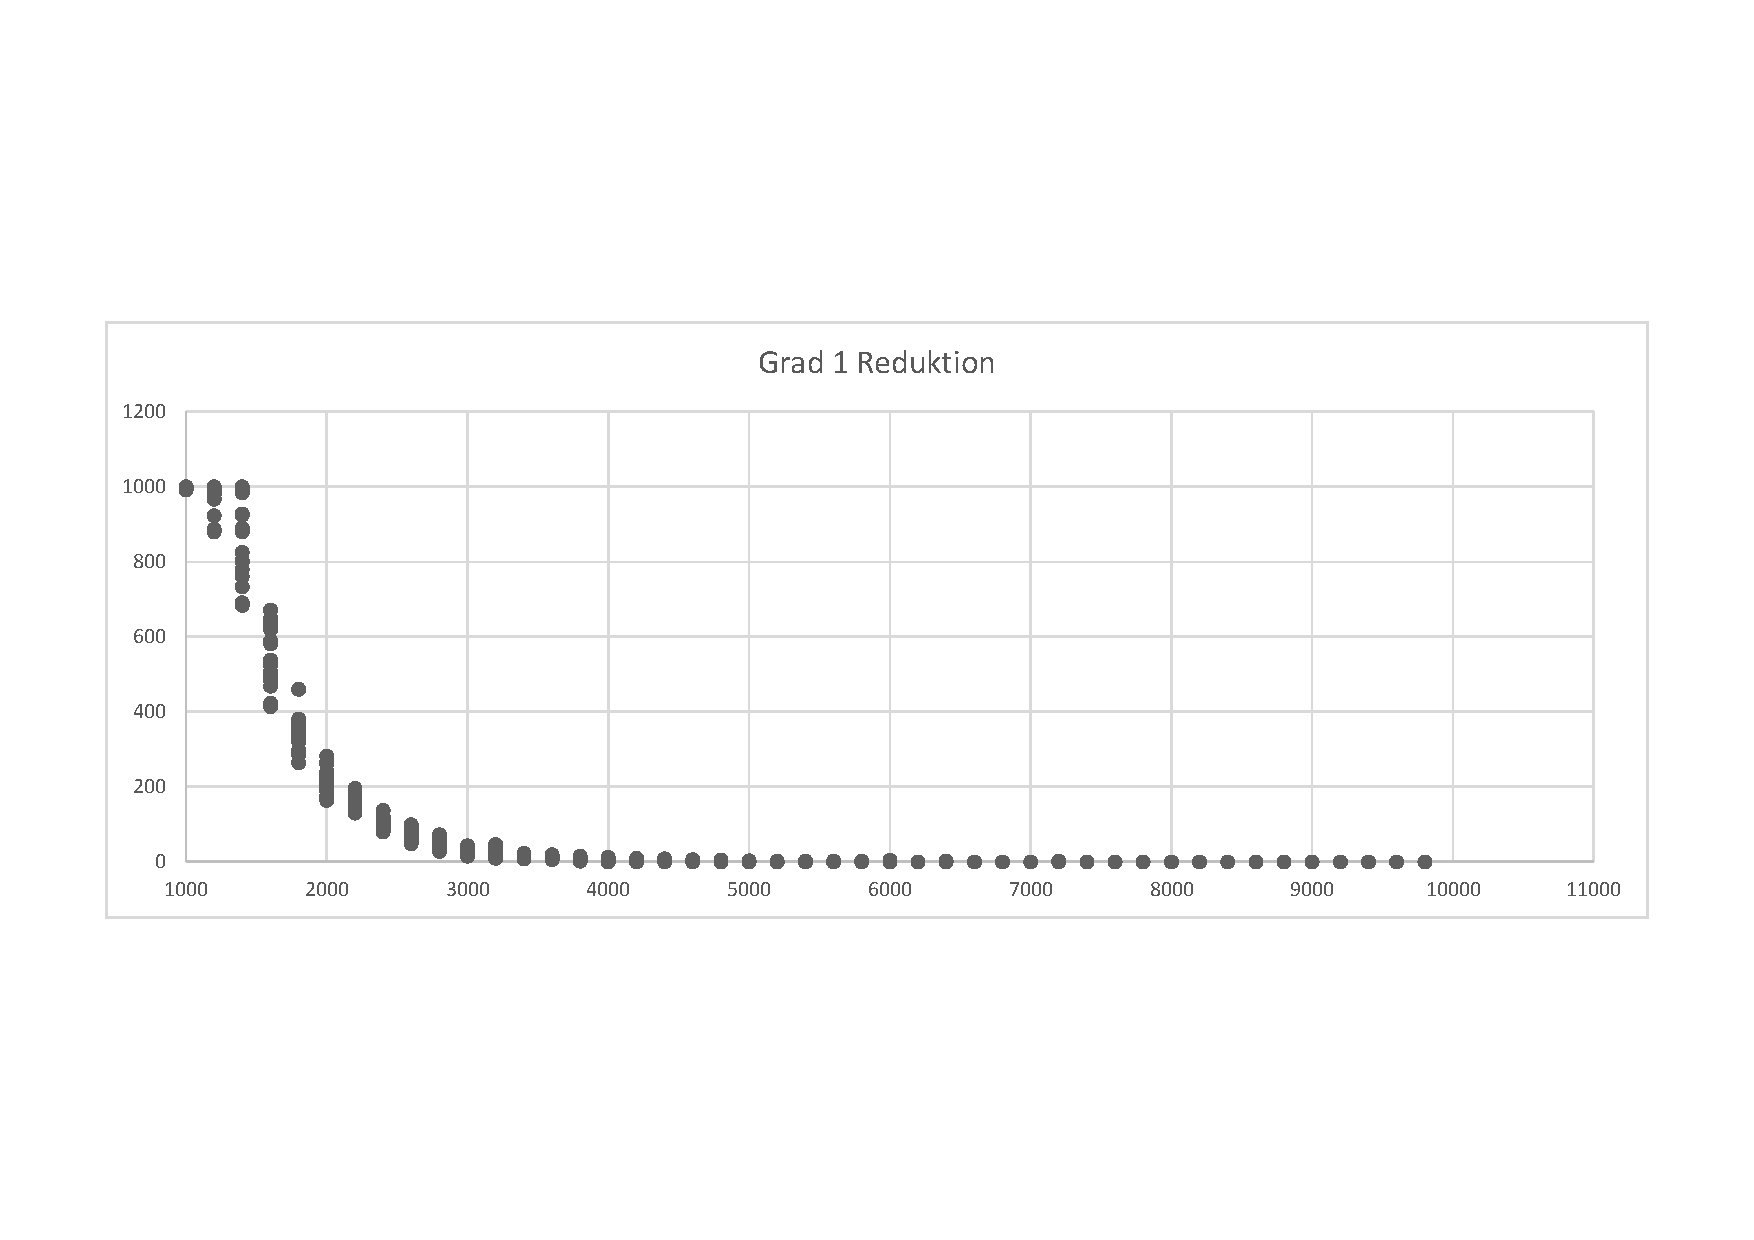
\includegraphics[scale= .4]{analysisOne.pdf} 
\end{frame}

\section{Kronenregel}

\begin{frame}{Kronenregel - Definitionen}
\begin{block}{Krone} 
\textit{Für einen Graphen} $G=(V,E)$ \textit{besteht eine Krone aus} $H \subseteq V\ und\ I \subseteq V\ mit\ H \cap I = \emptyset,\ sodass$  
\begin{enumerate}
\item $H = N(I),$  
\item $\forall v, w \in I\ gilt\ (vw) \notin E\ und$ 
\item \textit{die Kanten zwischen H und I enthalten ein Matching indem alle Knoten aus H enthalten sind.}
\end{enumerate}
\end{block}
\end{frame}

\begin{frame}[fragile]
\frametitle{Kronenregel - Algorithmus}
\begin{lstlisting}[mathescape=true, escapechar = !,basicstyle=\ttfamily\scriptsize]
$G = (V, E), n:= |V|, m:=|E|, d:= maximaler\ Grad\ eines\ Knoten\ aus\ G$
$M_{1}$ := Maximal Matching von $G$
  $M_{1} := \emptyset$
  $\forall e \in$ E:
    $M_{1} = M_{1} \cup e$
    Entferne $e$ und $N(e)$ aus der weiteren Betrachtung
$O$ := nicht gepaarte Knoten in $M_{1}$
$M_{2}$ := Maxmimum Matching von $B = (O, N(O), \{ uv| u \in O \wedge v \in N(O)\}) $
$I$  := nicht gepaarte Knoten aus $O$ in $M_{2}$
$I'  := \emptyset$
while $I' \neq I$
  $I' := I$
  $H:= N(I)$
  $I := I \cup \{\forall u \in O|\exists v\in H\ (uv \in M_{2})\}$
Entferne $N(I)$ aus $G$
\end{lstlisting}
\end{frame}

\begin{frame}[fragile]
\frametitle{Kronenregel - Laufzeit}
\begin{lstlisting}[mathescape=true, escapechar = !,basicstyle=\ttfamily\scriptsize]
$G = (V, E), n:= |V|, m:=|E|, d:= maximaler\ Grad\ eines\ Knoten\ aus\ G$
$M_{1}$ := Maximal Matching von $G$
  $M_{1} := \emptyset$
  $\forall e \in$ E:
    $M_{1} = M_{1} \cup e$
    Entferne $e$ und $N(e)$ aus der weiteren Betrachtung
$O$ := nicht gepaarte Knoten in $M_{1}$
$M_{2}$ := Maxmimum Matching von $B = (O, N(O), \{ uv| u \in O \wedge v \in N(O)\}) $
$I$  := nicht gepaarte Knoten aus $O$ in $M_{2}$
$I'  := \emptyset$
while $I' \neq I$
  $I' := I$
  $H:= N(I)$
  $I := I \cup \{\forall u \in O|\exists v\in H\ (uv \in M_{2})\}$
Entferne $N(I)$ aus $G$
\end{lstlisting}
\only<1>{Zeilen 1-5: $m \cdot d$}
\only<2>{Zeile 6: $n$}
\only<3>{Zeile 7 (1): $n d/2$} % $(n-2k) d/2$
\only<4>{Zeile 7 (2): $\sqrt{n} \cdot m $ (LEDA:mcb\_matching, Hopcroft und Karp) } %$\sqrt{n-2k} \cdot m $
\only<5>{Zeile 8: $n$ } %$n-2k$
\only<6>{Zeilen 10-13: $n \cdot d$}%Nachgucken welche Knoten aus O noch in M2   $(n-2k) \cdot d$
\end{frame}
\begin{frame}{Kronenregel - Laufzeit}
\begin{align*}
&\ m \cdot d + n + n d/2 + \sqrt{n} \cdot m + n  + n \cdot d \\  
=&\ d (m+n) +2 n + nd/2 + \sqrt{n} \cdot m \\  
\Rightarrow &\ O(\sqrt{n} \cdot m)
\end{align*}
\end{frame}

\begin{frame}{Kronenregel - Besonderheiten}
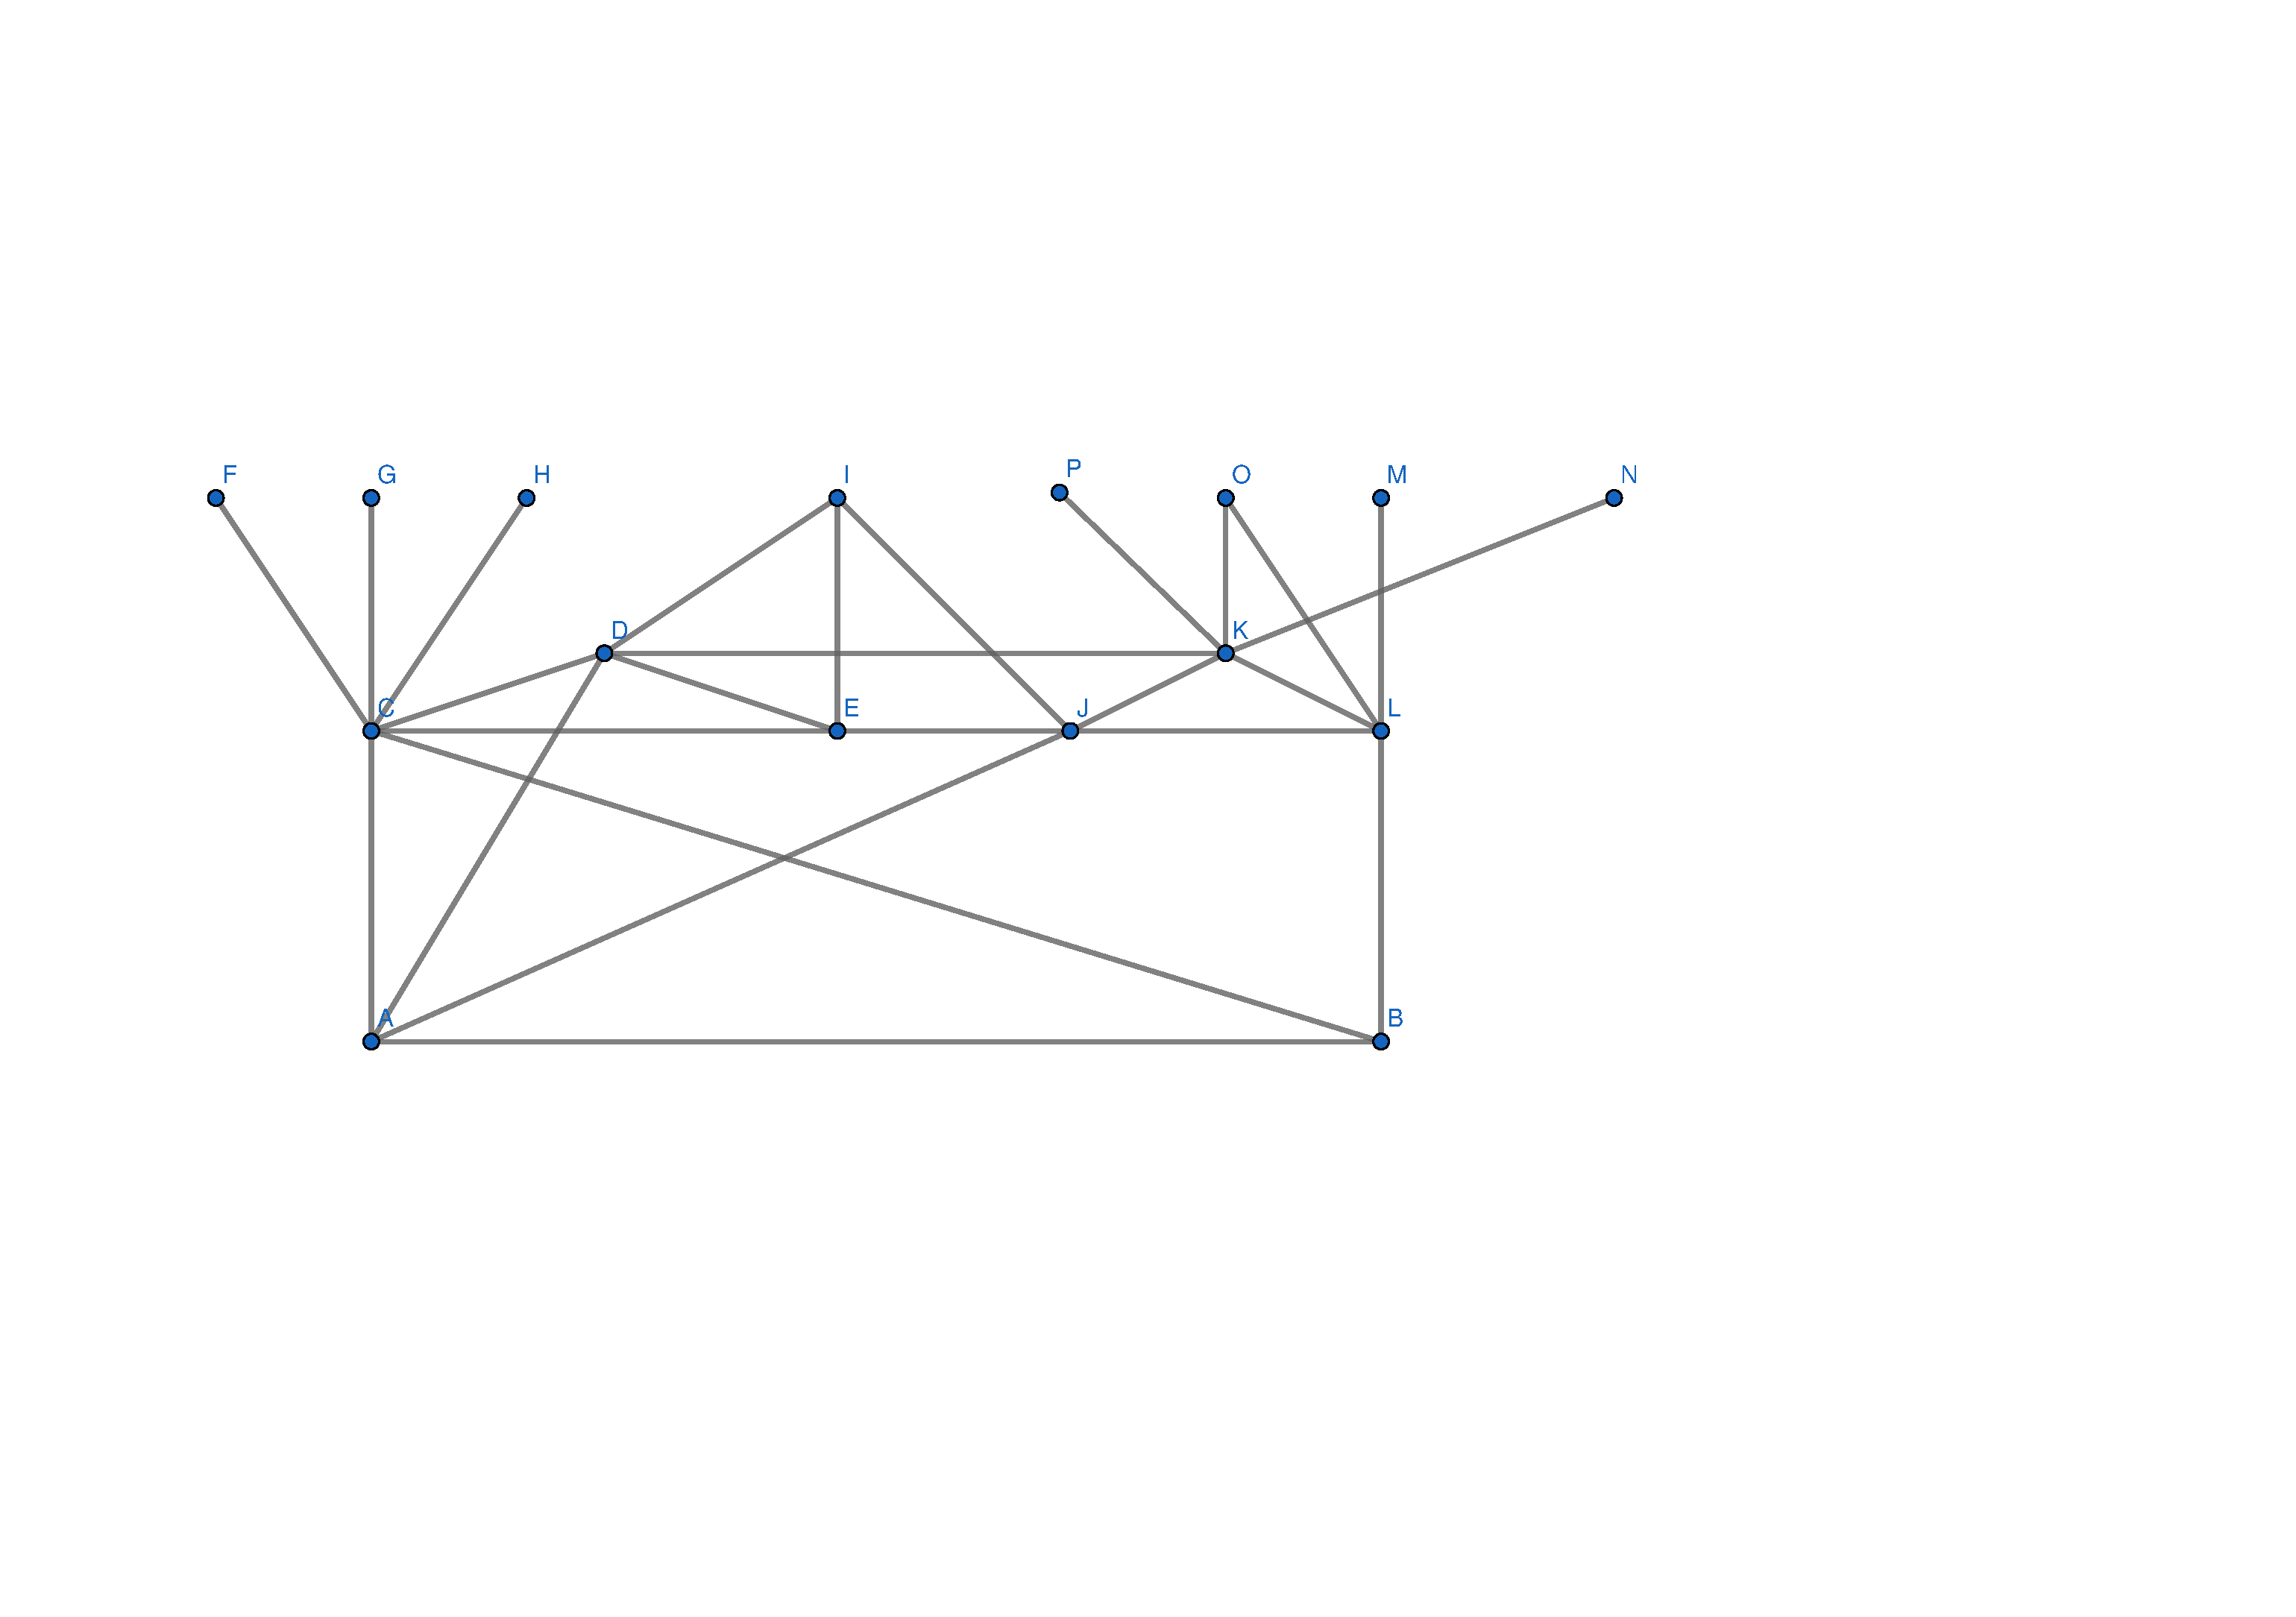
\includegraphics[scale=.3]{Crown1.pdf} 
\end{frame}
\begin{frame}{Kronenregel - Besonderheiten}
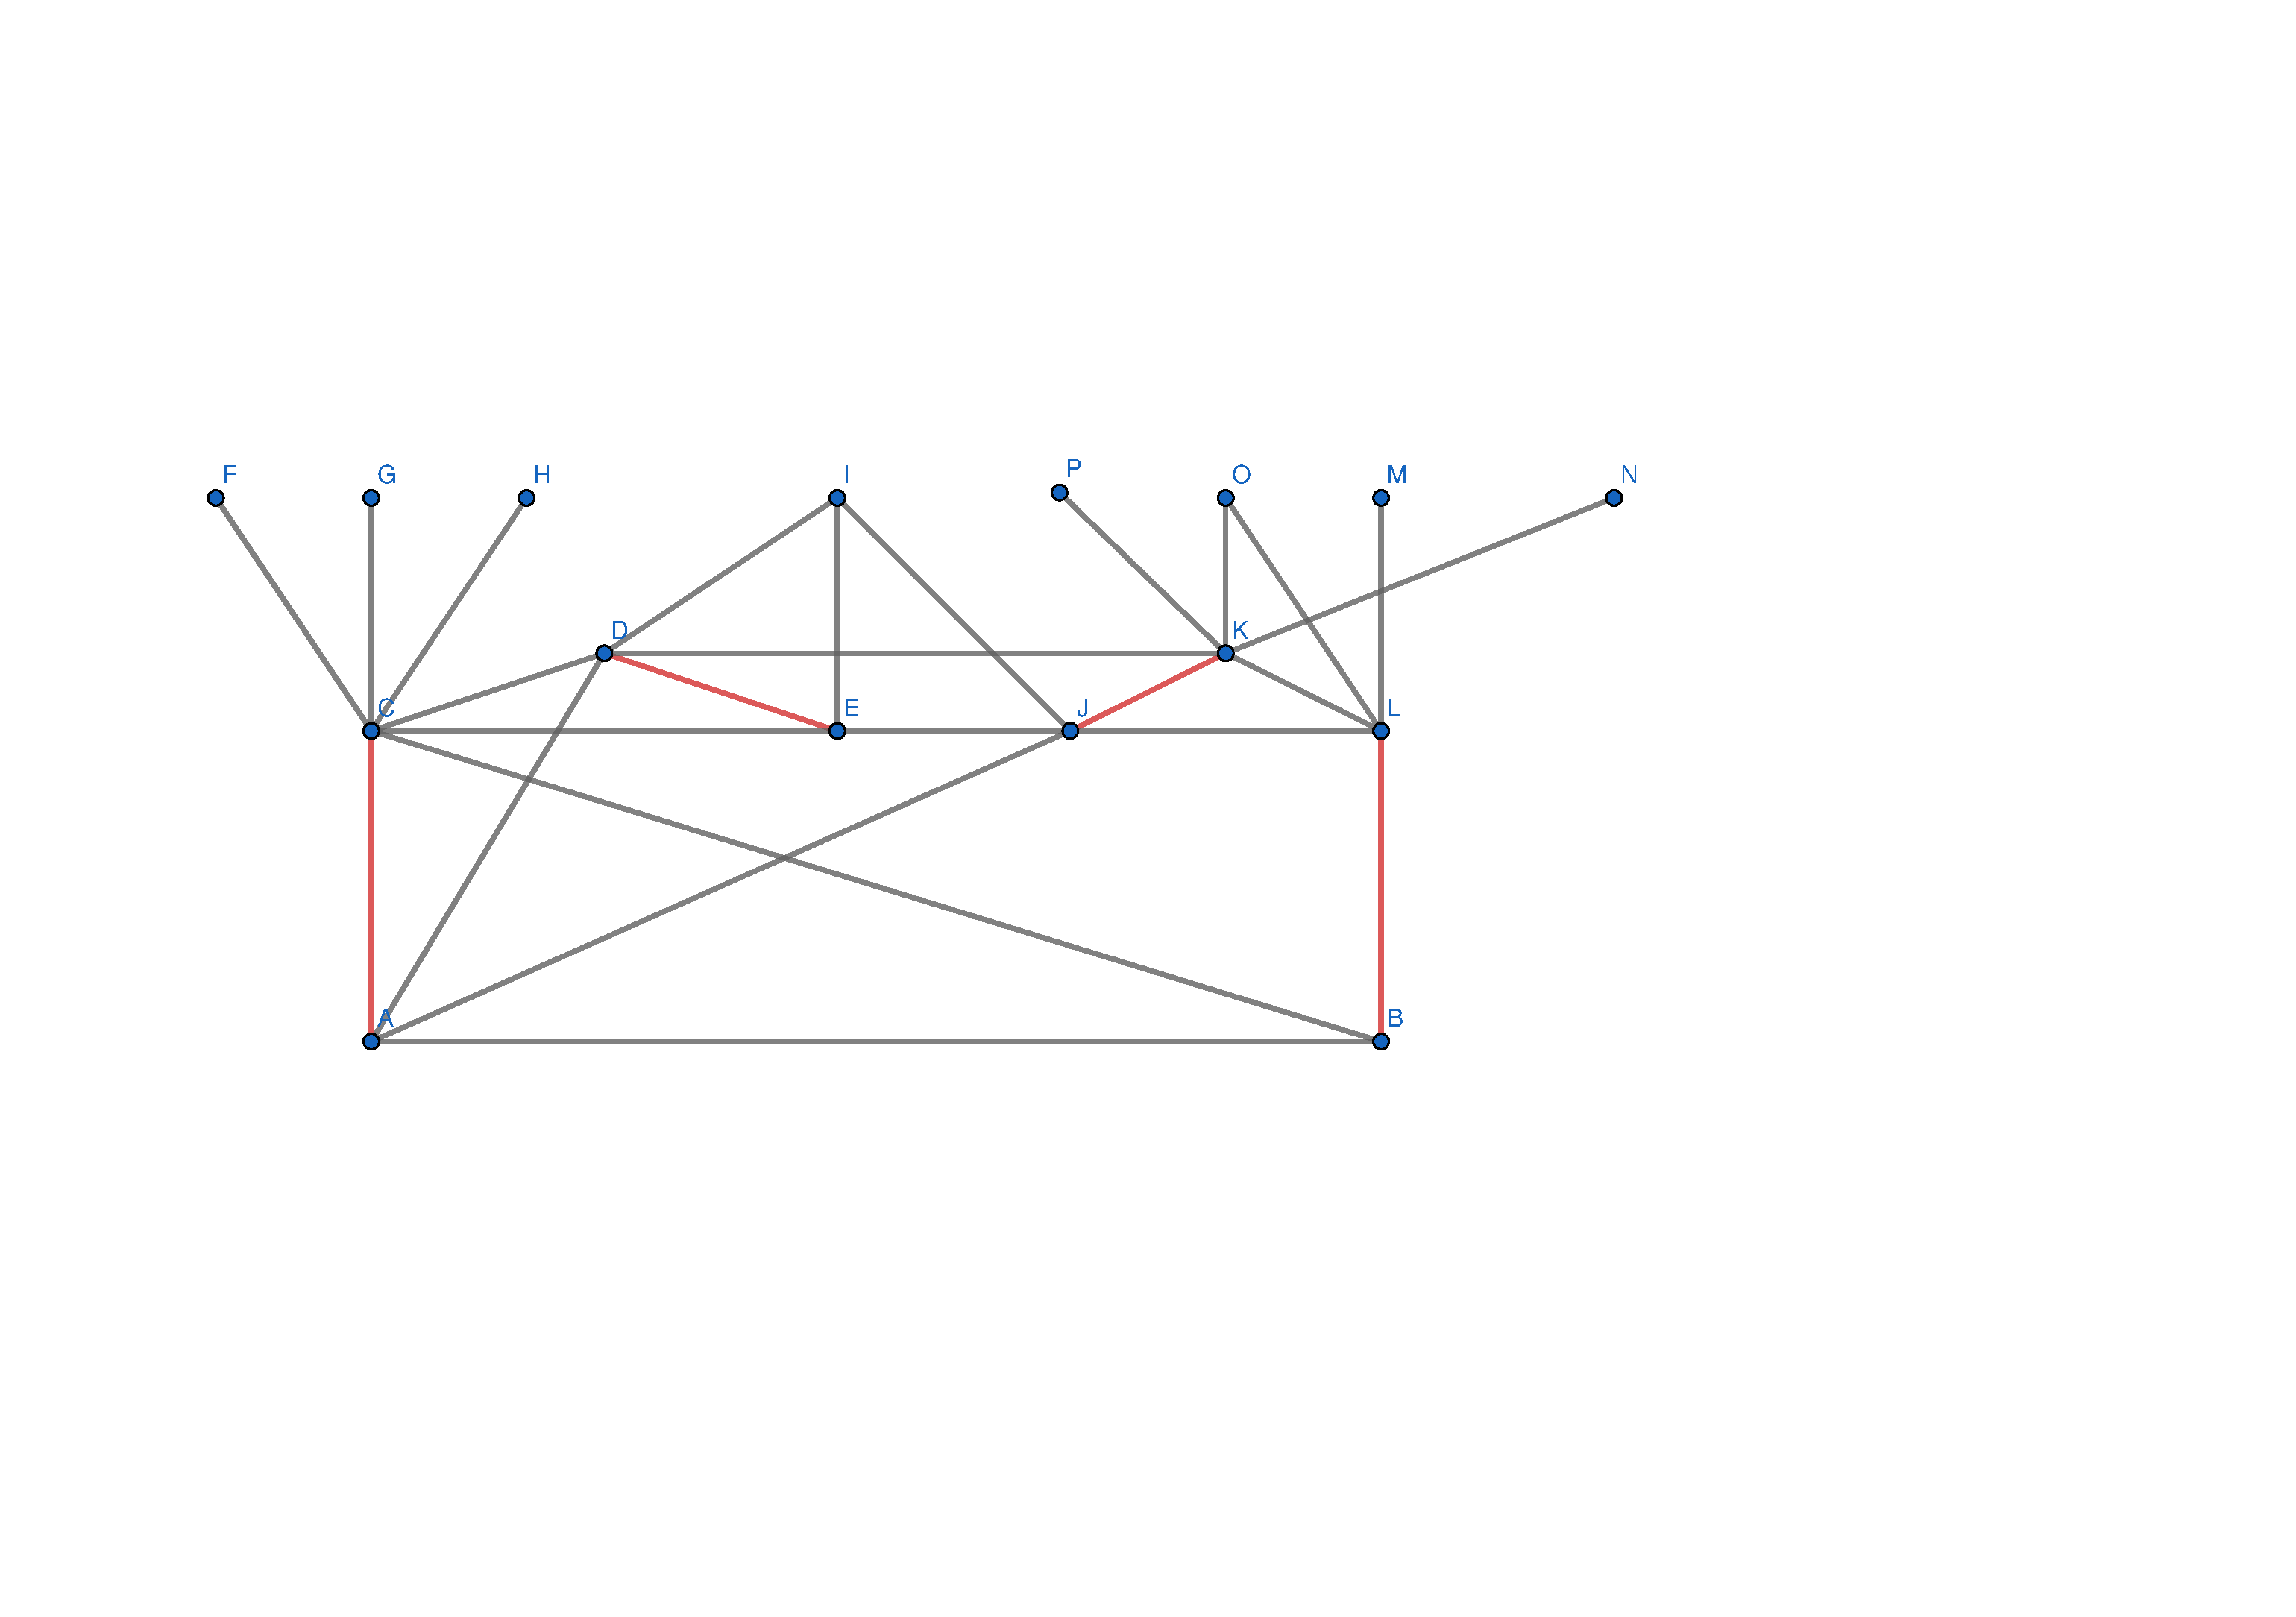
\includegraphics[scale=.3]{Crown2.pdf} 
\end{frame}
\begin{frame}{Kronenregel - Besonderheiten}

\begin{table}[htb]
\caption{Mindestens ein Knoten mit Einschränkung\label{tab:degreeOR}}
\vspace*{1em}
\centering

\bgroup
\def\arraystretch{1.3}%  1 is the default, change whatever you need


\begin{tabular}[c]{l|l|l}
	
	\multicolumn{1}{c|}{\textbf{Grad der Knoten}} & 
	\multicolumn{1}{c|}{\textbf{Anwendungen}} & 
	\multicolumn{1}{c}{\textbf{Reduktion}} \\ 
	
	\hline

	keine Einschränkung&0.29&13.04\\
	$>$1&0.29 &13.04 \\
	$>$2&0.29 &13.22 \\
	$>$3& 0.27& 12.92 \\
	$>$4& 0.3& 13.71 \\
	$>$5& 0.31&13.38 \\  
	$>$Größte Anzahl& 0.32&13.44 \\
	$>$Durchschnittliche Anzahl& 0.29&12.98 \\
	
\end{tabular}


\egroup

\end{table}

\end{frame}



\begin{frame}{Kronenregel - Besonderheiten}
\begin{table}[htb]
\caption{Beide Knoten mit Einschränkung\label{tab:degreeAND}}
\vspace*{1em}
\centering

\bgroup
\def\arraystretch{1.3}%  1 is the default, change whatever you need

\begin{tabular}[c]{l|l|l}
	
	\multicolumn{1}{c|}{\textbf{Grad der Knoten}} & 
	\multicolumn{1}{c|}{\textbf{Anwendungen}} & 
	\multicolumn{1}{c}{\textbf{Reduktion}} \\ 
	
	\hline

	keine Einschränkung&0.29&13.04\\
	$>$1&0.36 &15.34 \\
	$>$2&0.41 &16.96 \\
	$>$3& 0.39& 16.52 \\
	$>$4& 0.4 &15.78 \\
	$>$5& 0.4 & 15.72\\  
	$>$Größte Anzahl& 0.29 &13.06 \\
	$>$Durchschnittliche Anzahl& 0.46&19.77 \\
	
\end{tabular}
\egroup

\end{table}
\end{frame}

\begin{frame}{Kronenegel - Laufzeit}
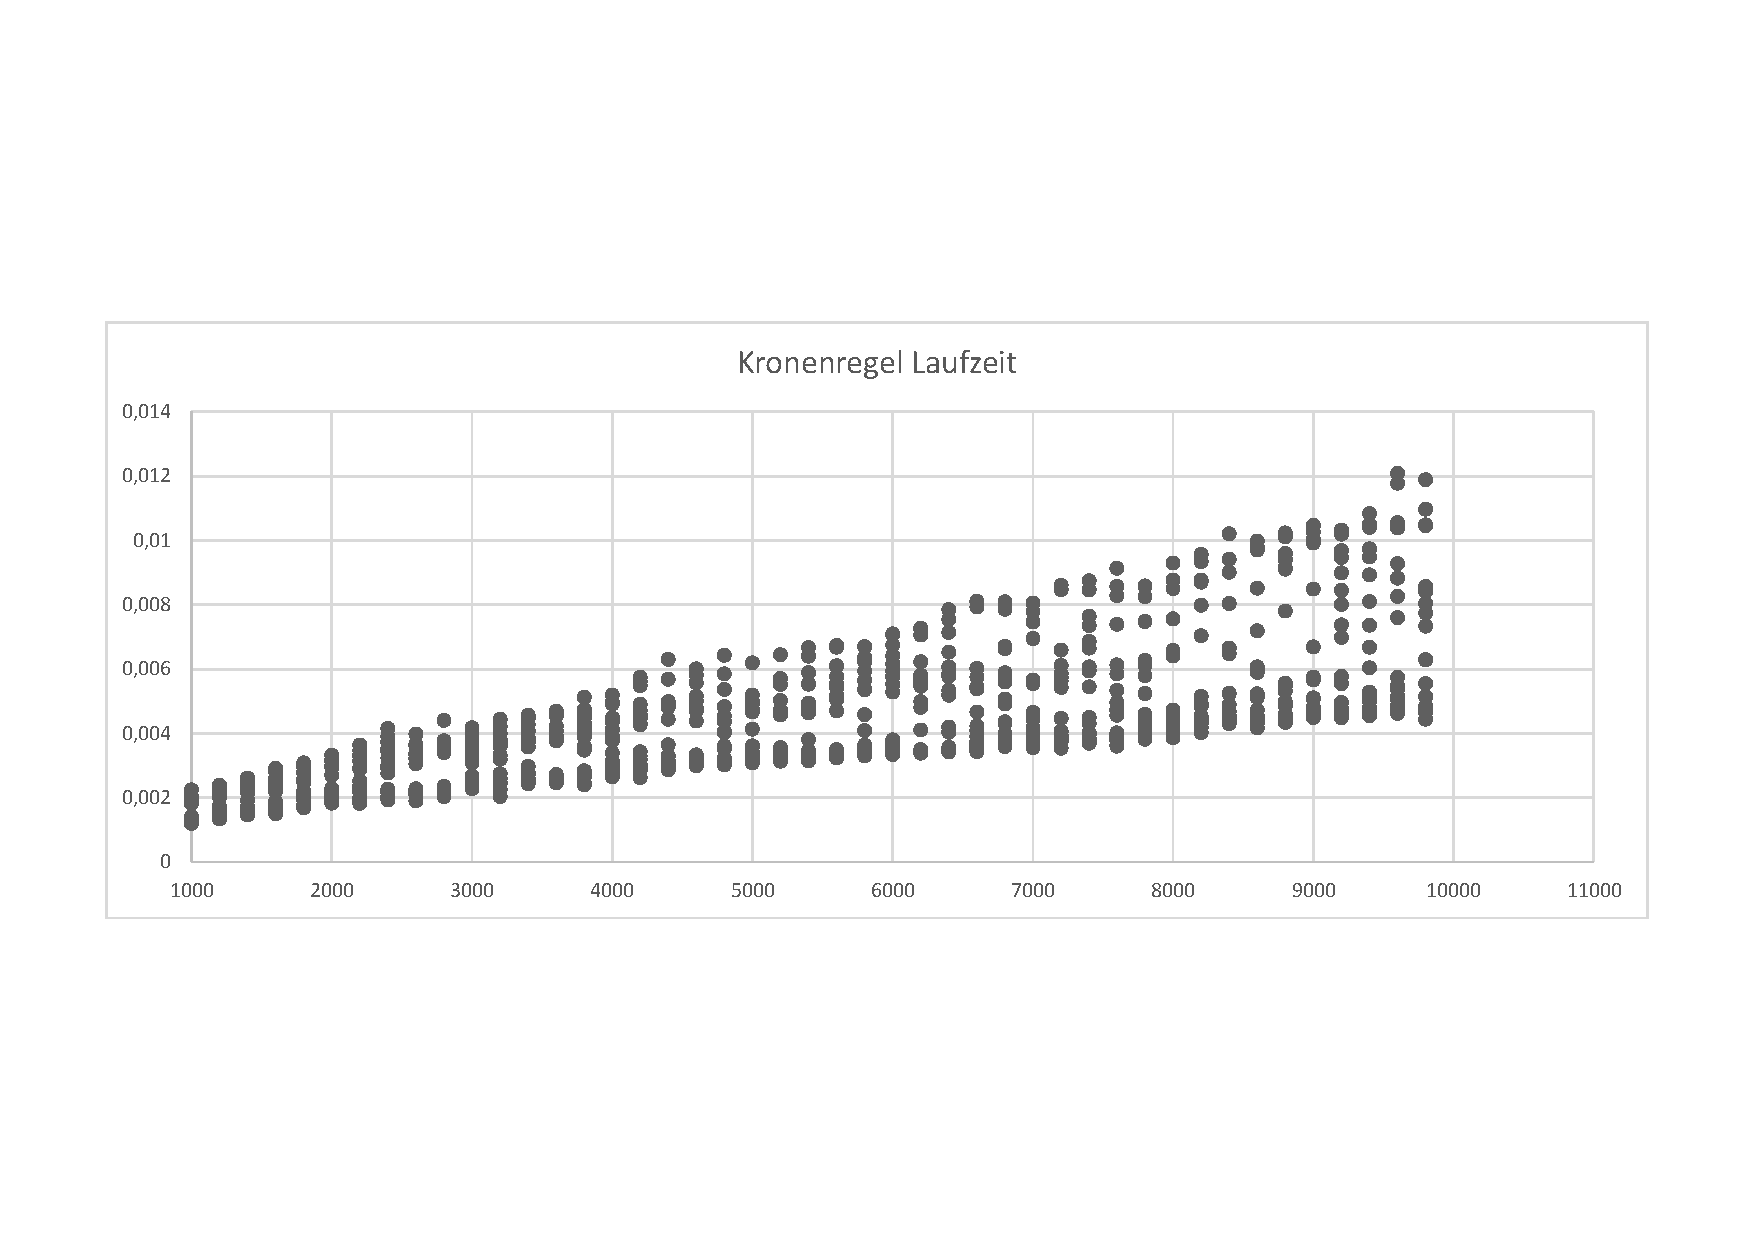
\includegraphics[scale= .4]{analysis1000_CrownNormal_runtime.pdf} 
\end{frame}

\begin{frame}{Kronenregel - Ergebnisse}
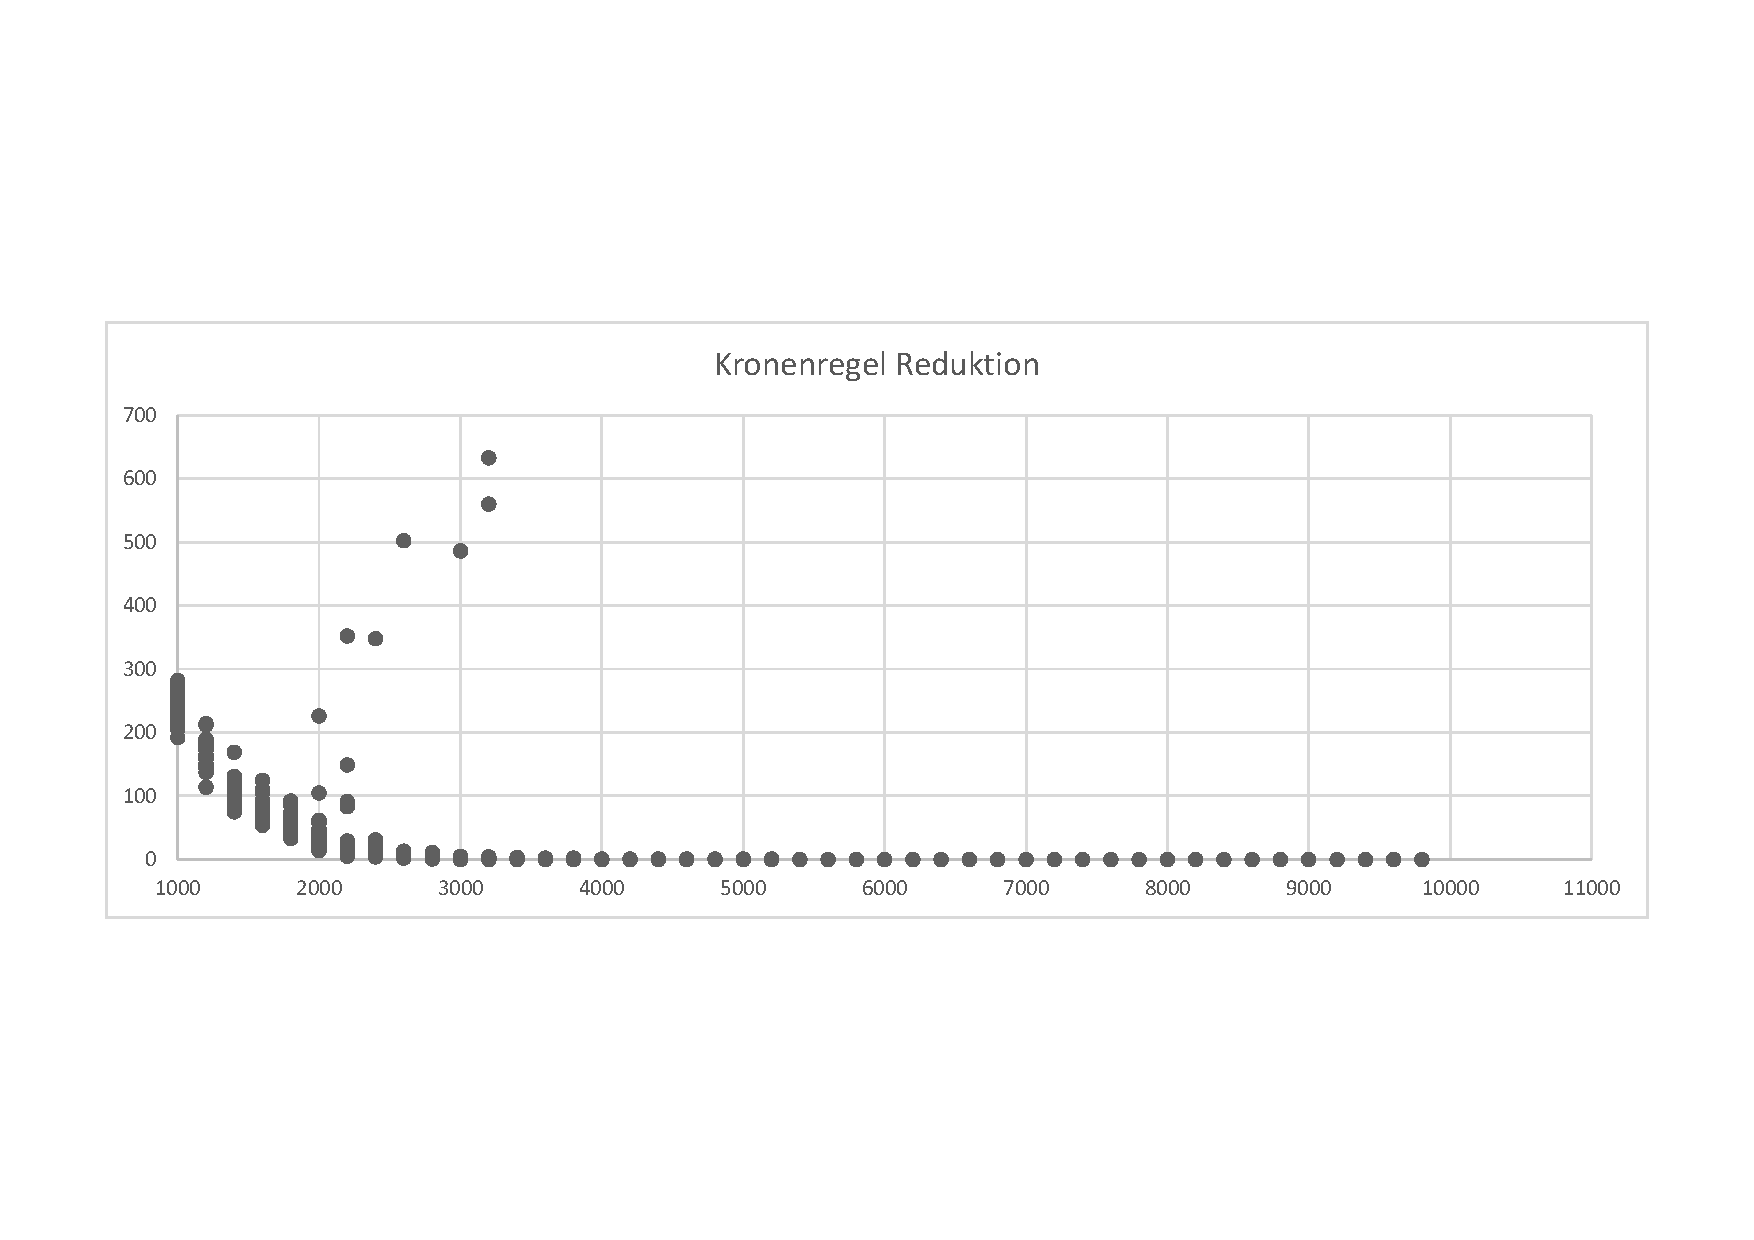
\includegraphics[scale= .4]{analysisCrown.pdf} 
\end{frame}

\section{Nemhauser-Trotter-Regel}
	
\begin{frame}{Nemhauser-Trotter-Regel}
\begin{block}{Nemhauser-Trotter-Theorem}
$\textit{Für einen Graphen}\ G=(V,E)\textit{ können zwei disjunkte Mengen}$\\ $\ C_{0}\ und\ V_{0} \textit{ gefunden werden, sodass}$ 
\begin{enumerate}
\item $C_{0}$ \textit{ in einer minimalen Knotenüberdeckung} \\
\textit{von G enthalten ist,} 
\item \textit{der Teilgraph }$G[V_{0}]$ \textit{eine Knotenüberdeckung}\\
\textit{der Größe} $\leq |V_{0}| / 2$ \textit{ hat,} 
\item \textit{und} $VC(G) = VC(G[V_{0}])\cup C_{0}$ \textit{ gilt.}
\end{enumerate}

\end{block}
\end{frame}
	
\begin{frame}[fragile]
\frametitle{NT-Regel - Algorithmus}
\begin{lstlisting}[mathescape = true, basicstyle=\ttfamily, escapechar = !]
$G = (V, E), n:= |V|, m:=|E|, d:= maximaler\ Grad\ eines\ Knoten\ aus\ G$
Bipartiden Graphen erstellen $B = (V, V', E')$
  mit $E':= \{\{x,y'\}, \{x', y\} | \{x,y\} \in E\}$
Maximum Matching $M$ von $B$ bestimmen
$C_{B}:= VC(B)$
$C_{0}:= \{x \in V\ |\ x \in C_{B}\ und\ x' \in C_{B} \}$
$V_{0}:= \{x \in V\ |\ entweder\ x \in C_{B}\ oder\ x' \in C_{B} \}$
\end{lstlisting}

\end{frame}

\begin{frame}[fragile]
\frametitle{NT-Regel - Laufzeit}
\begin{lstlisting}[mathescape = true, basicstyle=\ttfamily]
$G = (V, E), n:= |V|, m:=|E|, d:= maximaler\ Grad\ eines\ Knoten\ aus\ G$
Bipartiden Graphen erstellen $B = (V, V', E')$ 
  mit $E':= \{\{x,y'\}, \{x', y\} | \{x,y\} \in E\}$ 
Maximum Matching $M$ von $B$ bestimmen 
$C_{B}:= VC(B)$ 
$C_{0}:= \{x \in V\ |\ x \in C_{B}\ und\ x' \in C_{B} \}$ 
$V_{0}:= \{x \in V\ |\ entweder\ x \in C_{B}\ oder\ x' \in C_{B} \}$ 
\end{lstlisting}
\only<1>{Zeilen 1-2: $n \cdot 2d$}
\only<2>{Zeilen 3-4: $\sqrt{2n} \cdot 2m$ (LEDA:mcb\_matching, Hopcroft und Karp)}
\only<3>{Zeilen 5-6: $2n + k \cdot d$}
\end{frame}
\begin{frame}{NT-Regel - Laufzeit}
\begin{align*}
&\ n \cdot 2d + \sqrt{2n} \cdot 2m + 2n + k \cdot d\\  
\Rightarrow &\ O(n + \sqrt{n} \cdot m)
\end{align*}
\end{frame}


\begin{frame}{NT-Regel - Laufzeit}
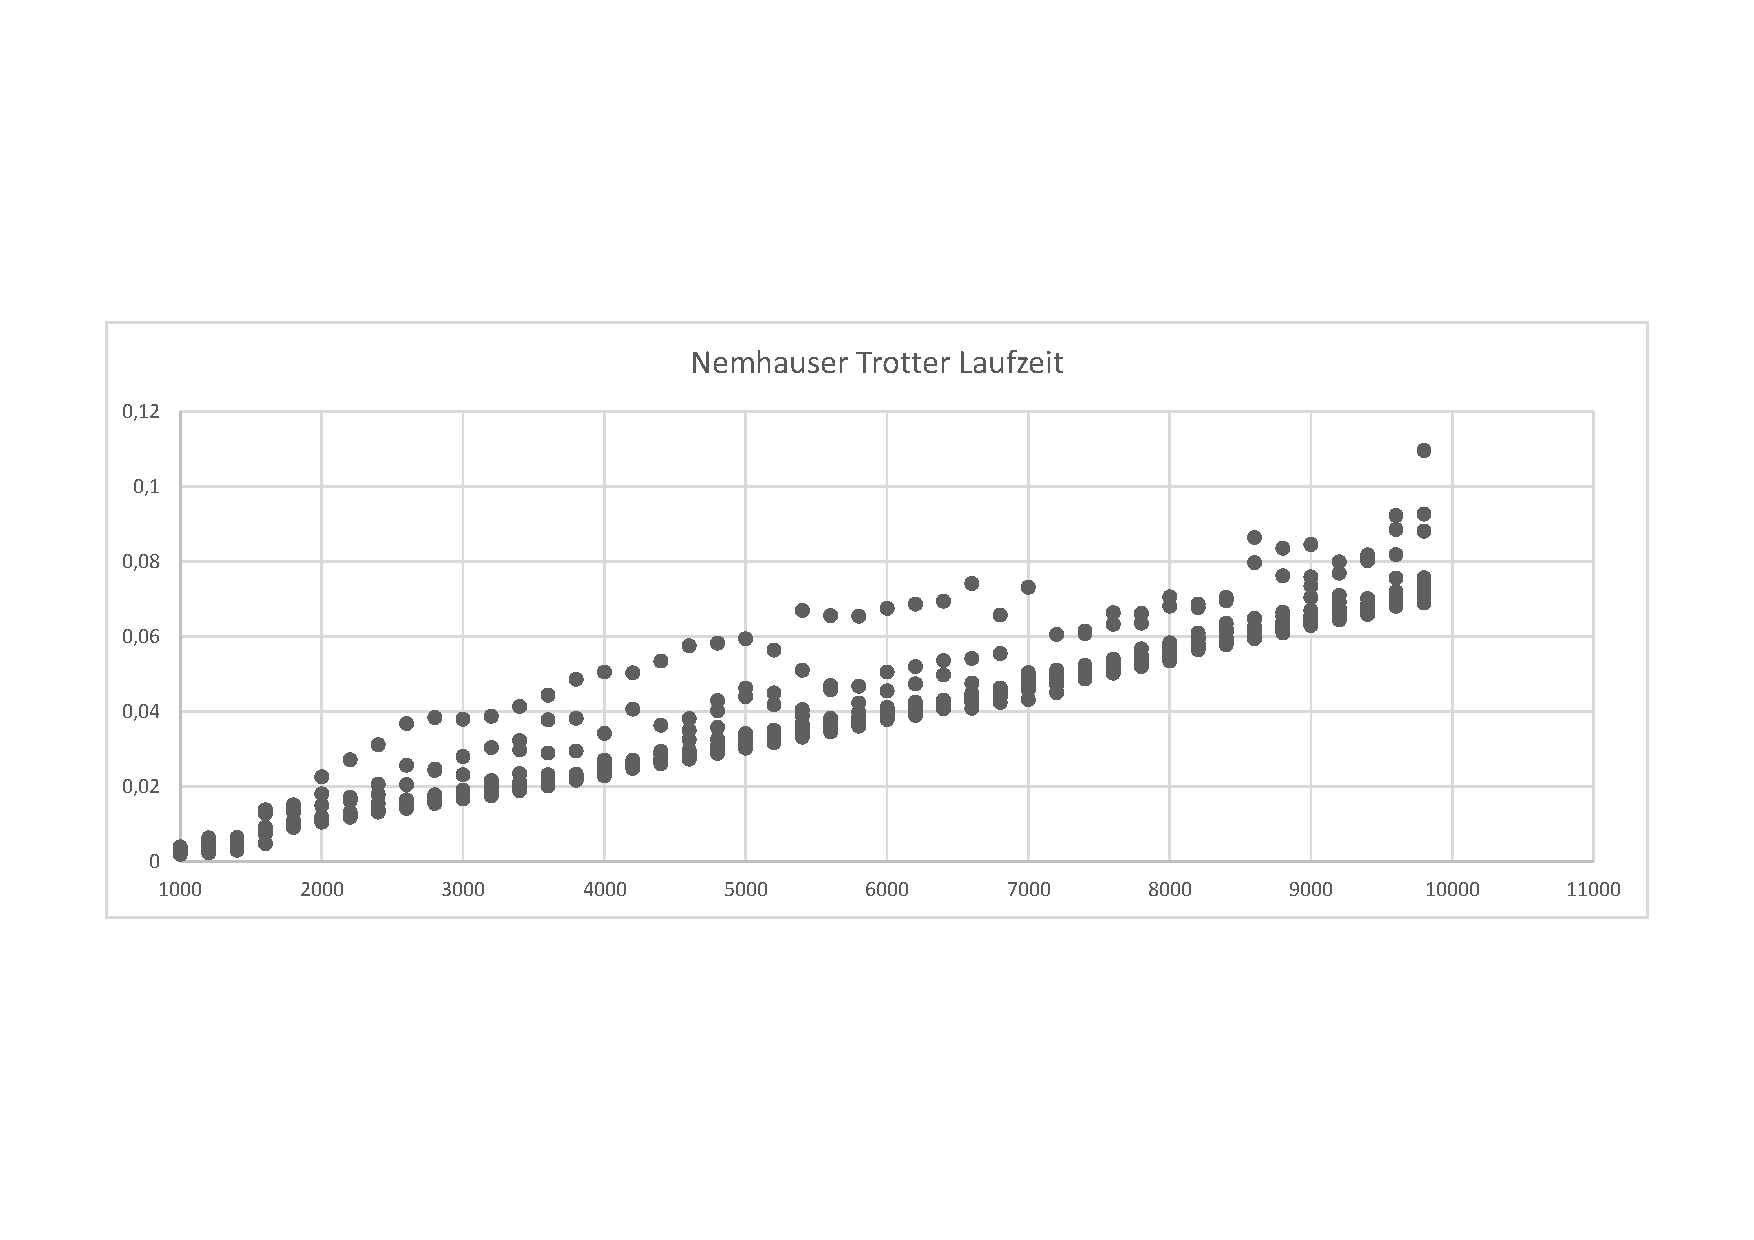
\includegraphics[scale= .4]{analysis1000_TrottNormal_runtime.pdf} 
\end{frame}
\begin{frame}{NT-Regel - Ergebnisse}
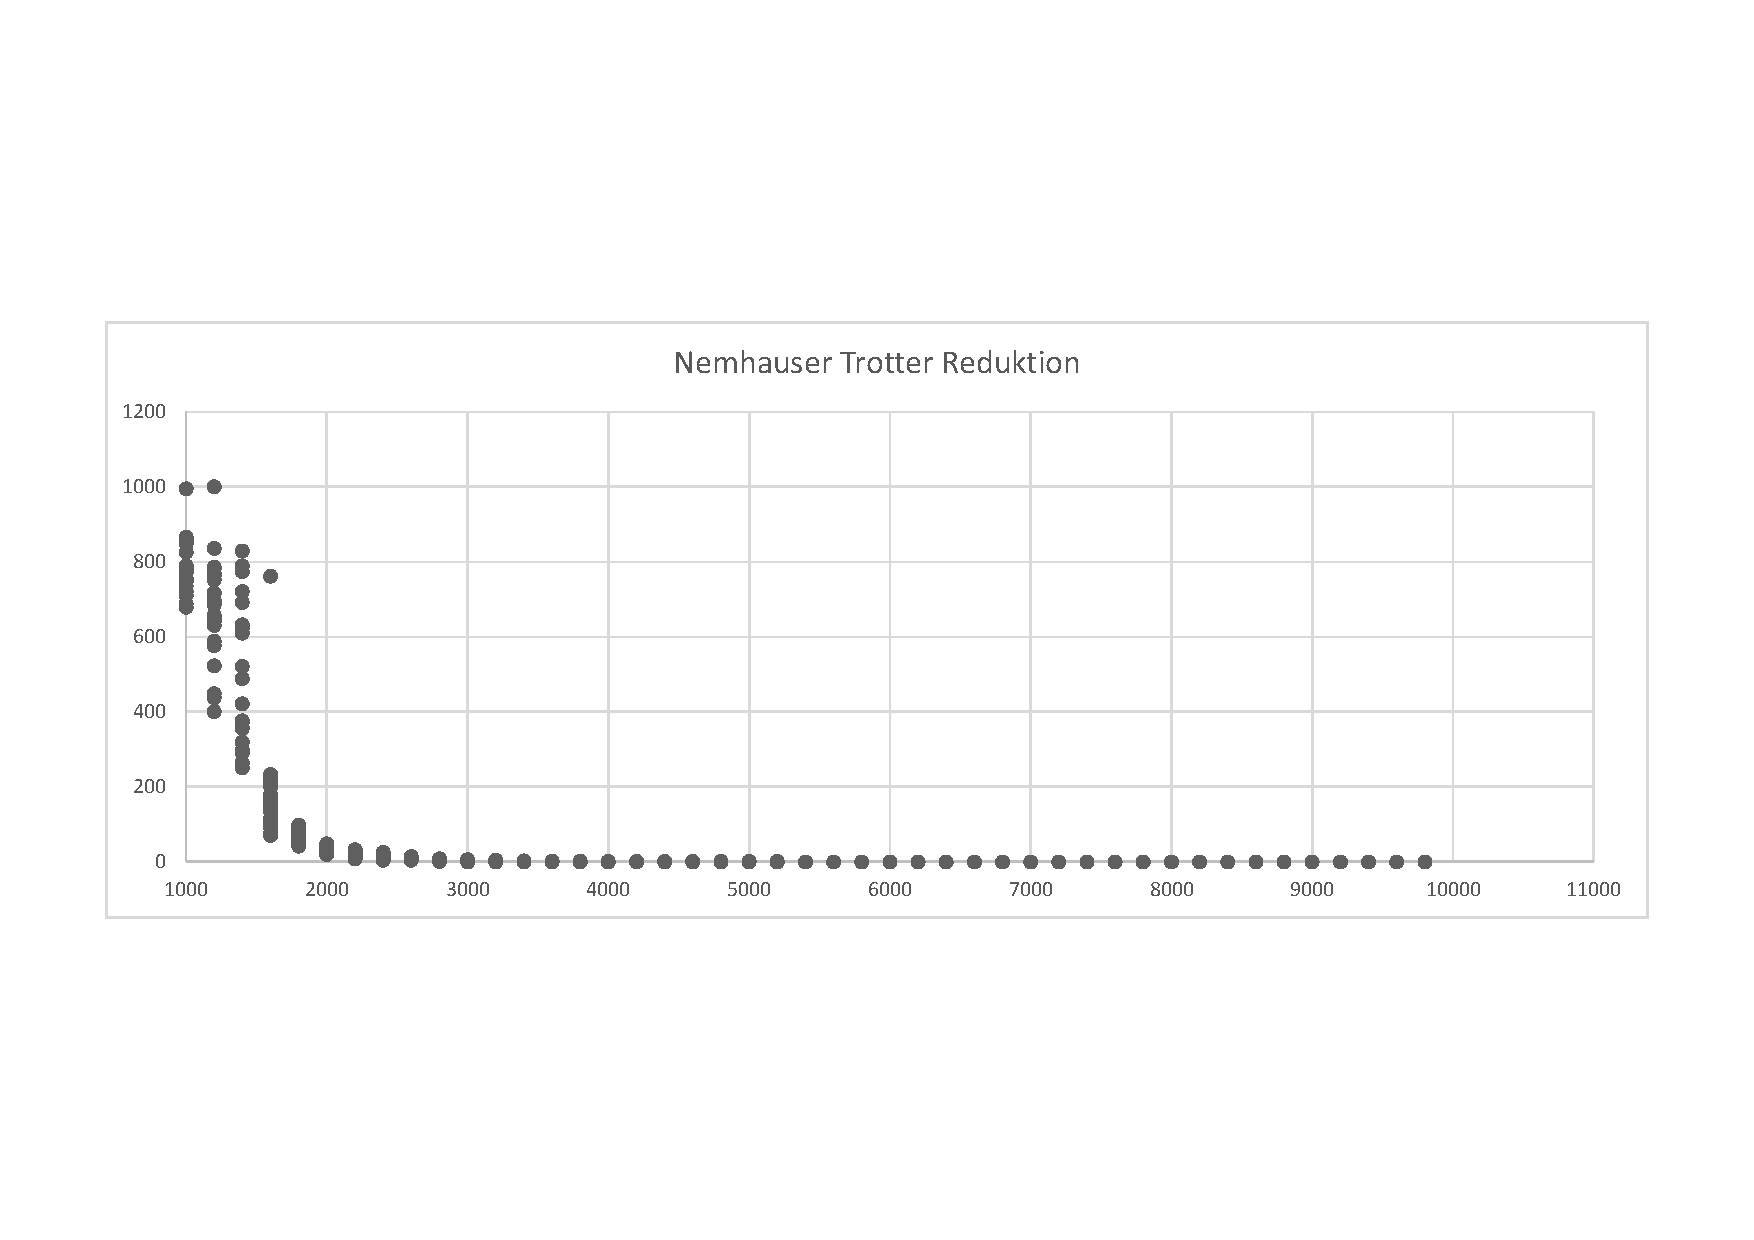
\includegraphics[scale= .4]{analysisTrott.pdf} 
\end{frame}

\section{Vergleich}
\begin{frame}{Vergleich der Ergebnisse}
\begin{table}[htb]
\caption{Anwendung einzelner Reduktionsregeln\label{tab:anwendung}}
\vspace*{1em}
\centering

\bgroup
\def\arraystretch{1.3}%  1 is the default, change whatever you need

\begin{tabular}[c]{llll}
	
	\hline
	\multicolumn{1}{c}{\textbf{Reduktionsregel}} & 
	\multicolumn{1}{c}{\textbf{Anwendungen}} & 
	\multicolumn{1}{c}{\textbf{Reduktion}} & 
	\multicolumn{1}{c}{\textbf{CPU-Zeit }} \\ 
	
	\hline

	Nemhauser-Trotter& 0.27 &  50.3 & 0.041s\\
	Kronenregel& 0.46 & 19.77 & 0.004s\\
	Grad 1&1.32 & 99.06 & 0.0006s\\
	\hline
\end{tabular}
\egroup

\end{table}
\end{frame}

\section{Anwendung}
\begin{frame}{Kombination}
\begin{table}[htbp]
\caption{Anwendung kombinierter Reduktionsregeln\label{tab:kombination}}
\vspace*{1em}
\centering

\bgroup
\def\arraystretch{1.3}%  1 is the default, change whatever you need
\resizebox{\linewidth}{!}{
\begin{tabular}[c]{lllll}

	\hline
	\multicolumn{1}{c}{\textbf{Kombination}} &
	\multicolumn{1}{c}{\textbf{Anwendungen$_{1}$}} &
	\multicolumn{1}{c}{\textbf{Anwendungen$_{2}$}} &
	\multicolumn{1}{c}{\textbf{Anwendungen$_{3}$}} & 
	\multicolumn{1}{c}{\textbf{Reduktion}} \\
	\hline

	\tikzmarkin<2>[hl]{a1}K - G{$_{1}$} & 3.63 & 4.3 & - &331.8\\
	\ G{$_{1}$} - K & 4.37 & 3.22 & - &331.17\tikzmarkend{a1}\\
	\tikzmarkin<4>[hl]{c1}K - NT & 0.8 & 0.38 & - & 68.28 \\
	\ NT - K & 0.45 & 0.56 & - & 68.6 \tikzmarkend{c1}\\
	\tikzmarkin<3>[hl]{b1}G{$_{1}$} - NT & 1.33 & 0.017 & - & 99.87\\
	\ NT - G{$_{1}$} & 0.28 & 1.13 & - & 99.87\tikzmarkend{b1}\\
	\hline
\end{tabular}
}
\egroup

\end{table}
\end{frame}
	\begin{frame}{Kombination}
\begin{table}[htbp]
\caption{Anwendung kombinierter Reduktionsregeln\label{tab:kombination}}
\vspace*{1em}
\centering

\bgroup
\def\arraystretch{1.3}%  1 is the default, change whatever you need
\resizebox{\linewidth}{!}{
\begin{tabular}[c]{lllll}

	\hline
	\multicolumn{1}{c}{\textbf{Kombination}} &
	\multicolumn{1}{c}{\textbf{Anwendungen{$_{1}$}}} &
	\multicolumn{1}{c}{\textbf{Anwendungen$_{2}$}} &
	\multicolumn{1}{c}{\textbf{Anwendungen$_{3}$}} & 
	\multicolumn{1}{c}{\textbf{Reduktion}} \\
	\hline
	
	\ K  - G{$_{1}$} - NT &\ 3.61 &\ 4.29 & 0.11 & 334.67\\ 
	\ K - NT - G{$_{1}$} & \tikzmarkin<2>[hl]{a2}3.6 &\ 0.87\tikzmarkend{a2} & 3.39 & 334.83 \\
	\ G{$_{1}$} - NT - K &\ 4.36 &\ 0.12 & 3.2 & 334.17 \\
	\ G{$_{1}$} - K - NT &\ 3.61 & \tikzmarkin<2>[hl]{b2}3.2 & 0.65\tikzmarkend{b2} & 334.16 \\
	\tikzmarkin<3>[hl]{d2}NT - K - G{$_{1}$} &\ 0.39 &\ 3.44 & 4.03 & 335.2 \tikzmarkend{d2} \\
	\ NT - G{$_{1}$} - K & \tikzmarkin<2>[hl]{c2}0.91 &\ 3.42 & 3.2\tikzmarkend{c2} & 334.16 \\
	\hline
	
\end{tabular}
}
\egroup
\end{table}
\end{frame}

\begin{frame}{Kombination}
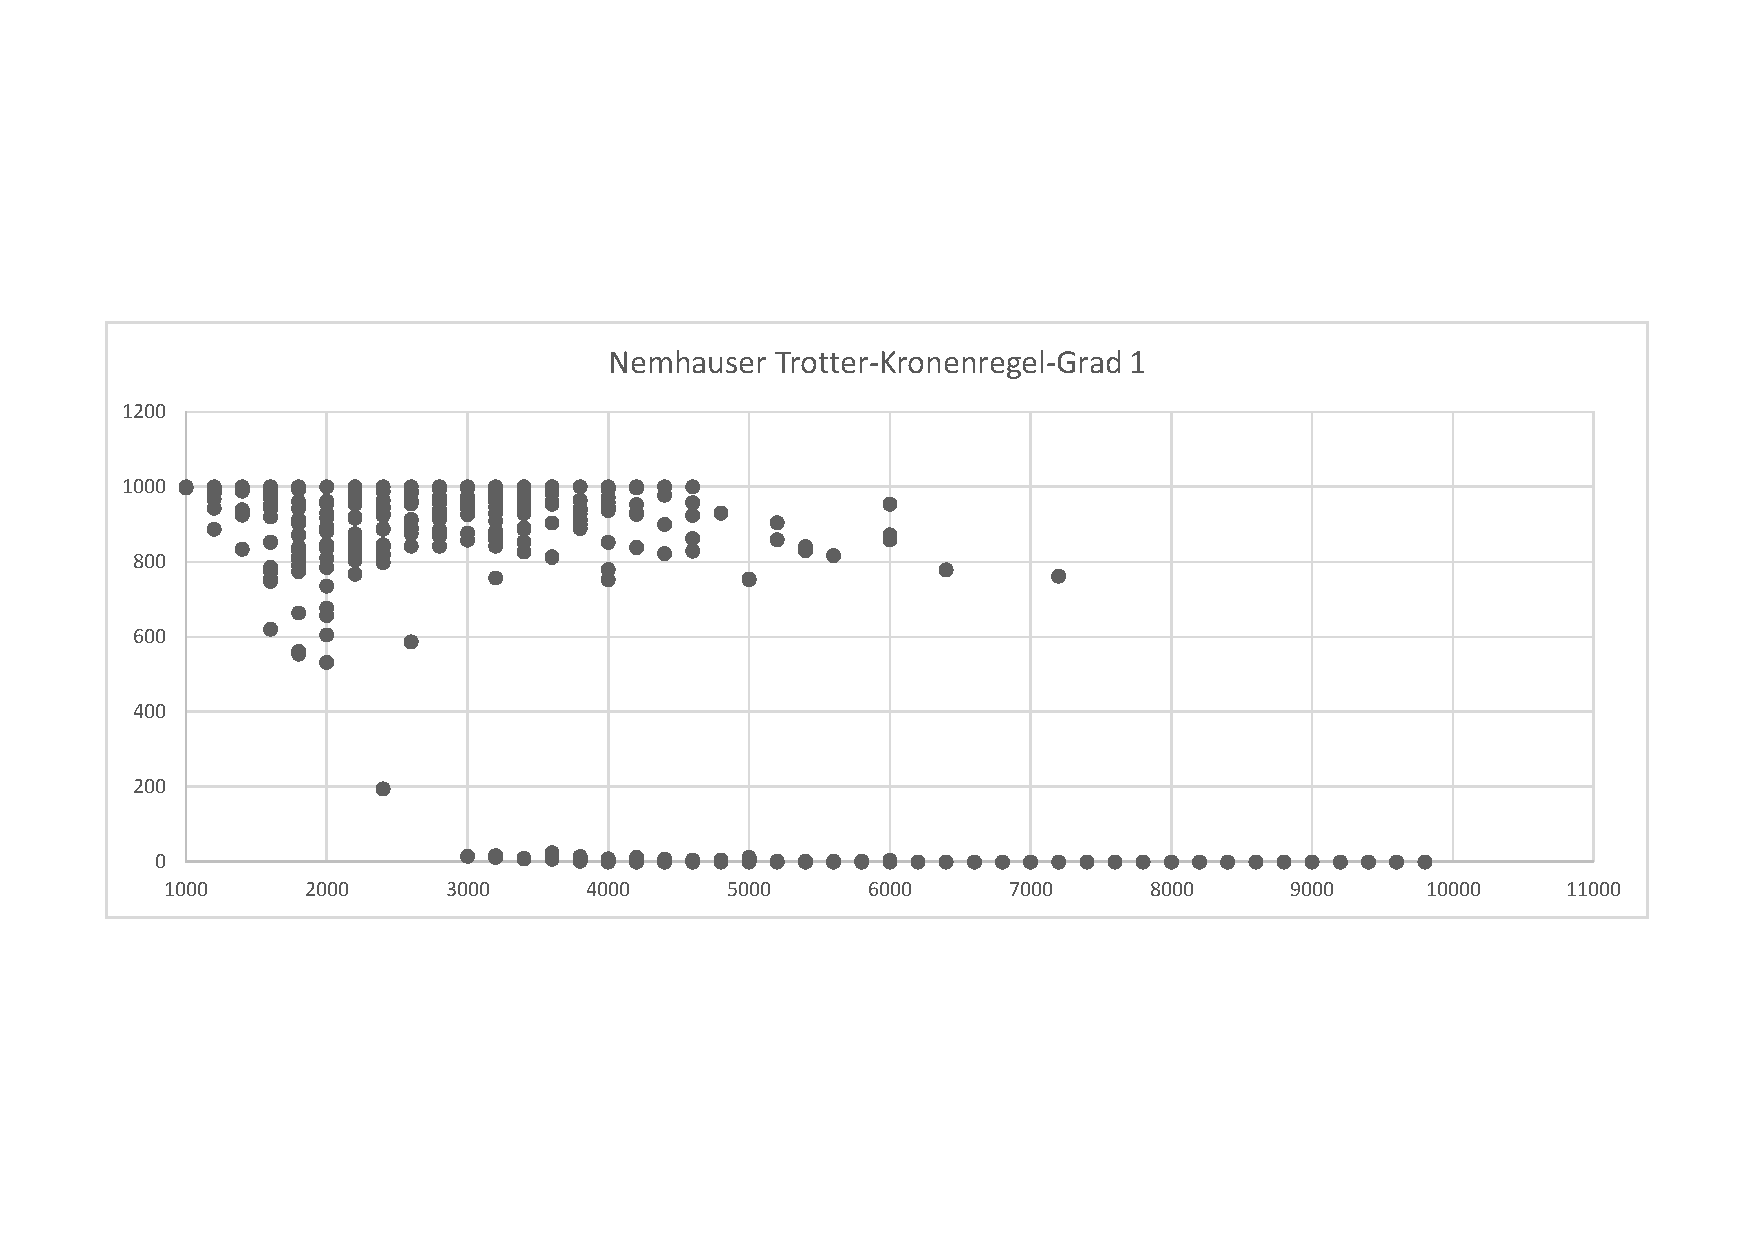
\includegraphics[scale=.4]{analysisTrott_Crown_One.pdf} 
\end{frame}

\begin{frame}{Kombination}
\begin{table}[htb]
\caption{Besondere Graphen für die Dreierkombinationen von Regeln\label{tab:trottCrownOneSpecial}}
\vspace*{1em}
\centering

\bgroup
\def\arraystretch{1.3}%  1 is the default, change whatever you need
\resizebox{.95\linewidth}{!}{
\begin{tabular}[c]{llllll}
	\hline
	\multicolumn{1}{c}{\textbf{Graph}} & 
	\multicolumn{1}{c}{\textbf{Reduktionsregeln}} & 
	\multicolumn{1}{c}{\textbf{Anwend.{$_{1}$}}} &
	\multicolumn{1}{c}{\textbf{Anwend.$_{2}$}} &
	\multicolumn{1}{c}{\textbf{Anwend.$_{3}$}} &
	\multicolumn{1}{c}{\textbf{Reduktion}} \\ 
	
	\hline
		
	Graph{$_{1}$} &\tikzmarkin<2>[hl]{b3}NT - K - G{$_{1}$} & 1 & 5 & 6 & 195  \tikzmarkend{b3} \\
	&\ G{$_{1}$} - NT - K & 6 & 0 & 5 & 195 \\
	&\ Nemhauser-Trotter & 1 & - & - & 11 \\
	&\ Kronenregel & 1 & - & - & 11 \\
	&\ Grad{$_{1}$} & 2 & - & - & 91 \\
	&\tikzmarkin<2>[hl]{a3}Kronenregel - Grad{$_{1}$} & 6 & 5 & - & 195 \tikzmarkend{a3}\\
	
	\hline

	Graph$_{2}$ &\ NT - K - G{$_{1}$} & 1 & 9 & 2 & 762 \\
	& \tikzmarkin<3>[hl]{c3}Nemhauser-Trotter & 0 & - & - & 0\\
	&\ Kronenregel & 0 & - & - & 0\\
	&\ Grad{$_{1}$} & 1 & - & - & 2\tikzmarkend{c3} \\
	&\ Kronenregel - Grad{$_{1}$} & 9 & 3 & - & 762\\
	\hline
	
\end{tabular}
}
\egroup

\end{table}

\end{frame}


\section{Fazit und Ausblick}
\begin{frame}{Fazit und Ausblick}
\begin{itemize}
\item Nehmhauser-Trotter-Regel, obwohl viel in der Literatur erwähnt liefert in der Praxis mäßige Ergebnisse $\Rightarrow$ Warum? 
	 \begin{itemize}
	\item Welche Form wäre für die Nemhauser Trotter am besten? 
	\end{itemize}
\item Wie ergibt sich in bei den Reduktionen mit Dreierkombination der Große Unterschied zwischen den Graphen im Bereich der Kantenmenge zwischen 3000 und 4600? 
\item Wieso ist das Matching M1 so wichtig für die Kronenregel? 
\end{itemize}
\end{frame}
  \begin{frame}[allowframebreaks]
        \frametitle{Quellen}
         % nur angeben, wenn auch nicht im Text zitierte Quellen 
           % erscheinen sollen
\bibliographystyle{ieeetran}
        \bibliography{thesis.bib}
\end{frame}
\end{document}